
\section{Introduction}

\subsection{Task}

In this project we compare Kernel Support Vector Machines (KSVMs) and state of the art techniques
like Convolutional Neural Networks (CNNs) for image classification.\\
Since image classification is a multi-class problem,
we implement our own strategies of how to use KSVMs in order to decide which class
will be assigned to a given image, and we compare our strategies to the strategies
which are implemented in the R-library \textit{kernlab}.\\
Both CNNs and KSVMs have a lot of parameters, so a main part of our work
was to search for parameter settings that lead to good classification results.


\subsection{Datasets}

We have three different datasets with varying kinds of images, image sizes and dataset sizes.


\subsubsection{ZIP}

The ZIP dataset was provided in the second part of the course for some homeworks.\\
It contains 16x16-pixel grayscale images of handdrawn digits from 0 to 9.
The dataset is rather small with a training set of 7291 and a test set of 2007 images.
See Figure \ref{zip_dataset} for example images.

\begin{figure}
 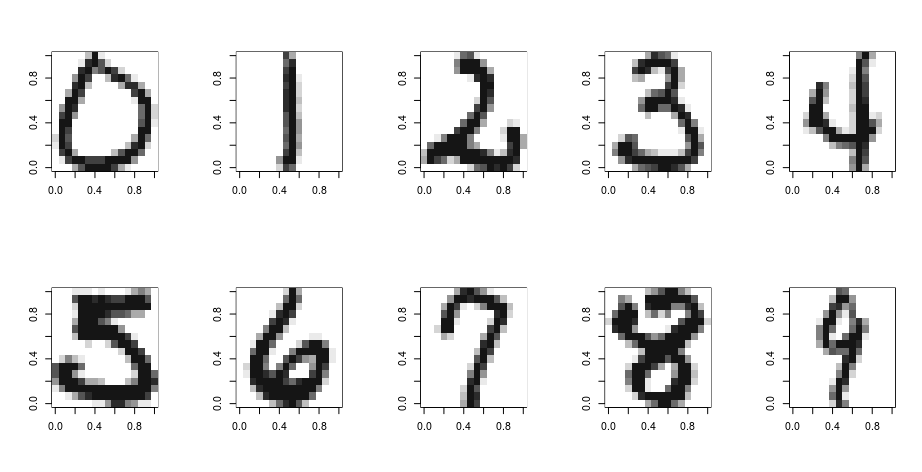
\includegraphics[width=\textwidth]{../plots/zip_dataset}
 \caption{Example images of the 10 classes of the ZIP dataset.}
 \label{zip_dataset}
\end{figure}


\subsubsection{MNIST}

The MNIST dataset is frequently used in the image classification literature
and can be considered to be a standard dataset.
We downloaded the dataset from \cite{mnist}.\\
It contains 28x28-pixel grayscale images of handdrawn digits from 0 to 9.
The dataset is bigger than the ZIP dataset and comes with a training set of 60000 and a test set of 10000 images.
See Figure \ref{mnist_dataset} for example images.\\

\begin{figure}
 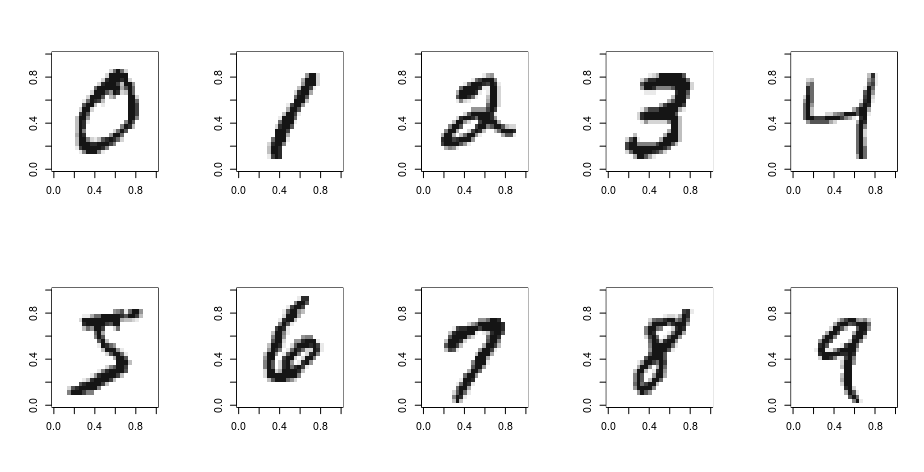
\includegraphics[width=\textwidth]{../plots/mnist_dataset}
 \caption{Example images of the 10 classes of the MNIST dataset.}
 \label{mnist_dataset}
\end{figure}


\subsubsection{CIFAR-10}

The CIFAR-10 dataset contains 32x32-pixel RGB-coloured images of the following ten classes
(see Figure \ref{cifar10_dataset} for example images):
\begin{enumerate}
 \item airplane
 \item automobile
 \item bird
 \item cat
 \item deer
 \item dog
 \item frog
 \item horse
 \item ship
 \item truck
\end{enumerate}

The dataset is divided into a training set of 50000 and a test set of 10000 images.\\
All the data can be found on \cite{cifar10}.

\begin{figure}
 \begin{minipage}{0.19\textwidth}
  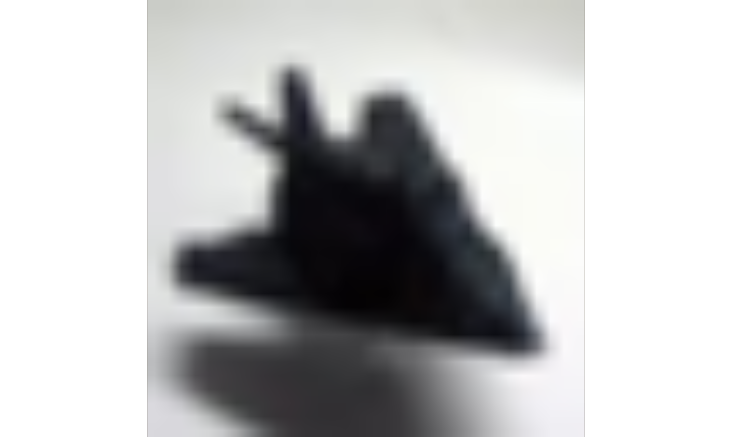
\includegraphics[width=1.5\textwidth]{../plots/cifar10-class0}
 \end{minipage}
 \begin{minipage}{0.19\textwidth}
  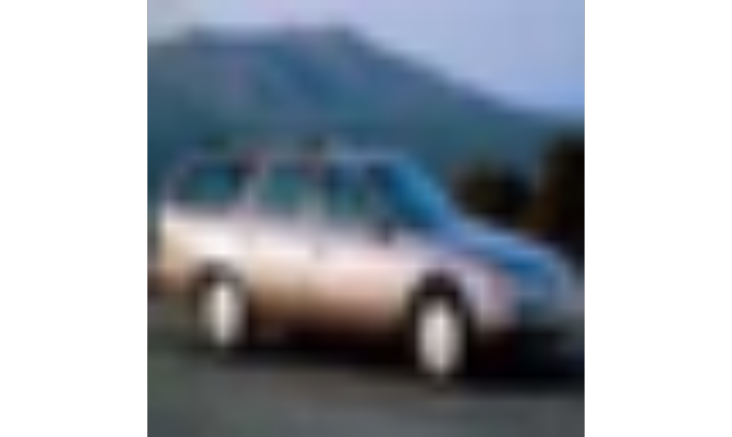
\includegraphics[width=1.5\textwidth]{../plots/cifar10-class1}
 \end{minipage}
 \begin{minipage}{0.19\textwidth}
  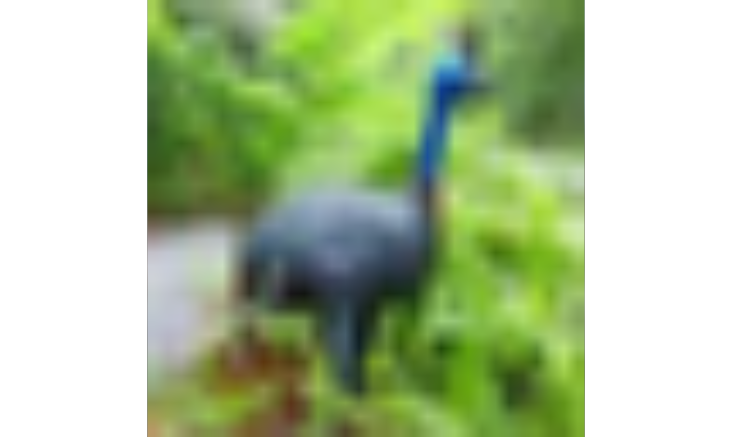
\includegraphics[width=1.5\textwidth]{../plots/cifar10-class2}
 \end{minipage}
 \begin{minipage}{0.19\textwidth}
  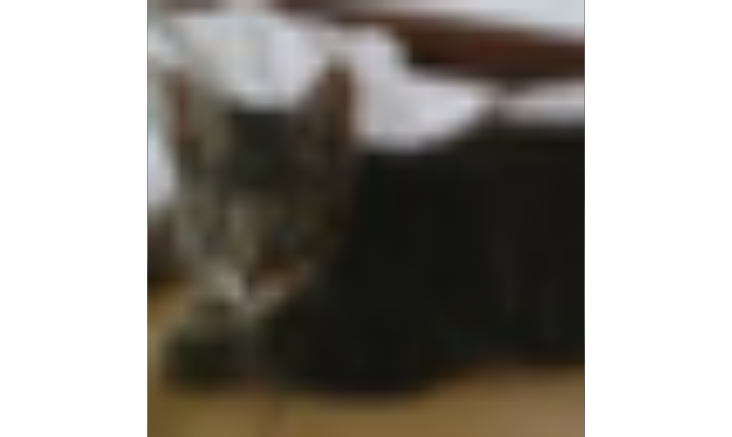
\includegraphics[width=1.5\textwidth]{../plots/cifar10-class3}
 \end{minipage}
 \begin{minipage}{0.19\textwidth}
  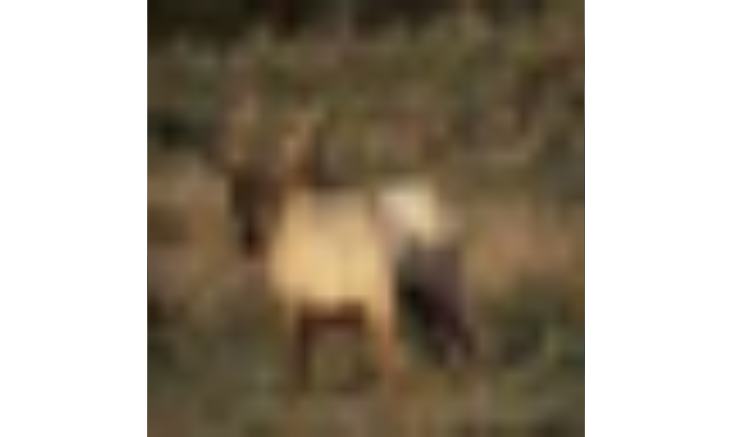
\includegraphics[width=1.5\textwidth]{../plots/cifar10-class4}
 \end{minipage}
 \begin{minipage}{0.19\textwidth}
  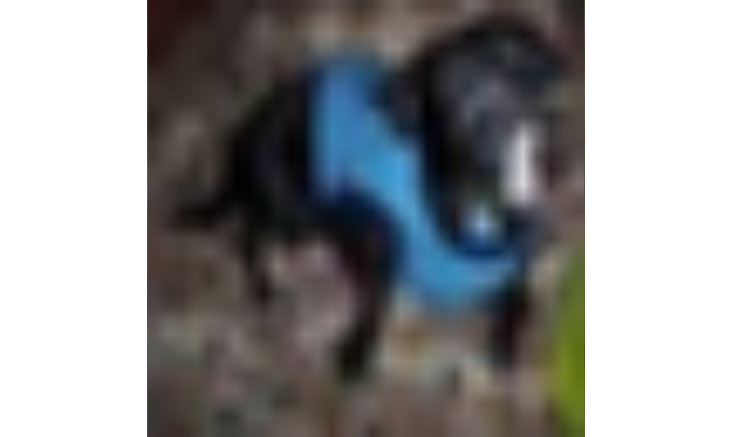
\includegraphics[width=1.5\textwidth]{../plots/cifar10-class5}
 \end{minipage}
 \begin{minipage}{0.19\textwidth}
  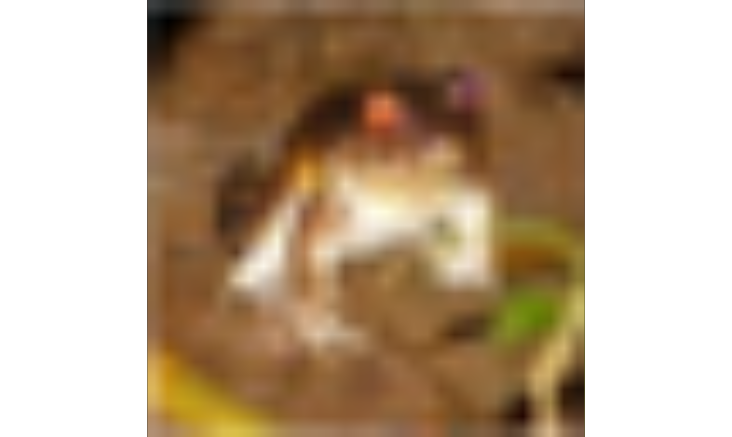
\includegraphics[width=1.5\textwidth]{../plots/cifar10-class6}
 \end{minipage}
 \begin{minipage}{0.19\textwidth}
  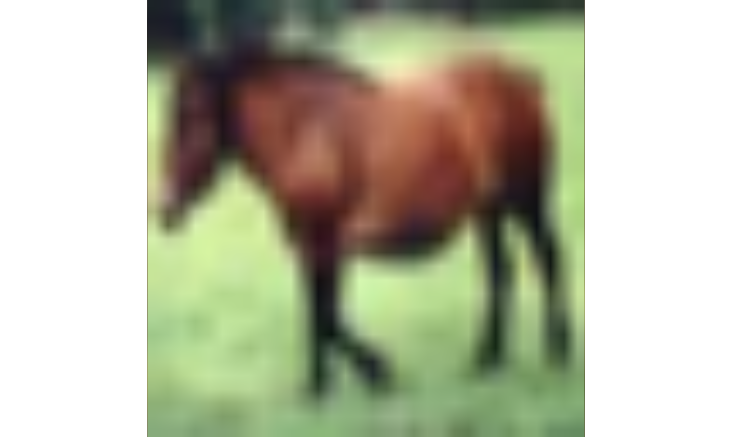
\includegraphics[width=1.5\textwidth]{../plots/cifar10-class7}
 \end{minipage}
 \begin{minipage}{0.19\textwidth}
  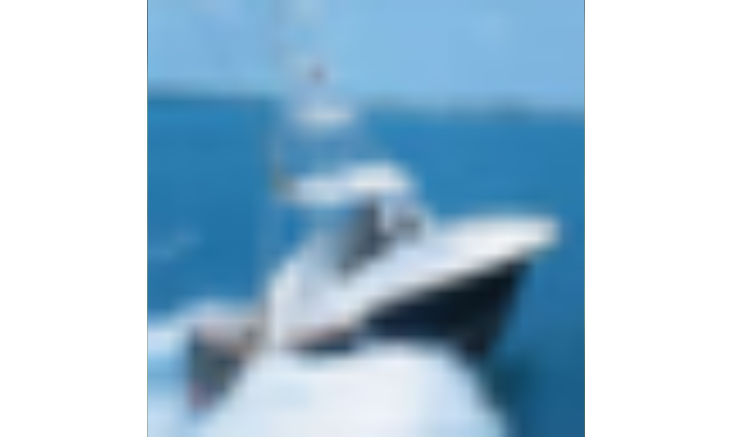
\includegraphics[width=1.5\textwidth]{../plots/cifar10-class8}
 \end{minipage}
 \begin{minipage}{0.19\textwidth}
  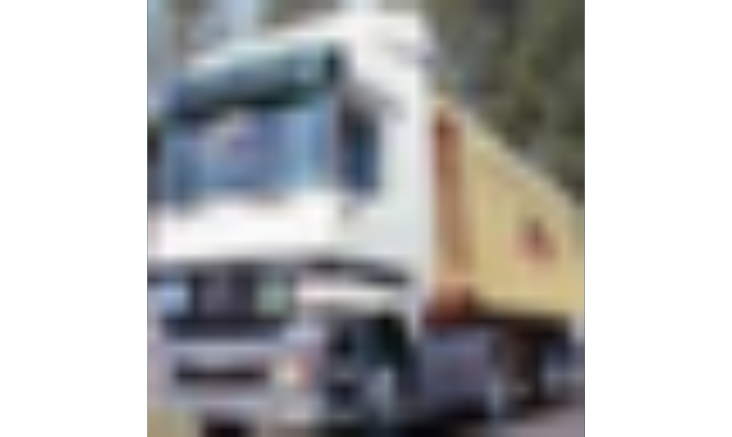
\includegraphics[width=1.5\textwidth]{../plots/cifar10-class9}
 \end{minipage}
 \caption{Example images for the 10 classes of the CIFAR-10 dataset.}
 \label{cifar10_dataset}
\end{figure}
